
%(BEGIN_QUESTION)
% Copyright 2011, Tony R. Kuphaldt, released under the Creative Commons Attribution License (v 1.0)
% This means you may do almost anything with this work of mine, so long as you give me proper credit

Examine the state of this fluid-heating system:

$$\includegraphics[width=15.5cm]{i00010x01.eps}$$

The temperature of the exiting fluid is well below setpoint, so we know there is a problem somewhere in this system.  

Determine the diagnostic value of each of the following tests.  Assume only one fault in the system, including any single component or any single wire/cable/tube connecting components together.  If a proposed test could provide new information to help you identify the location and/or nature of the one fault, mark ``yes.''  Otherwise, if a proposed test would not reveal anything relevant to identifying the fault (already discernible from the measurements and symptoms given so far), mark ``no.''

% No blank lines allowed between lines of an \halign structure!
% I use comments (%) instead, so that TeX doesn't choke.

$$\vbox{\offinterlineskip
\halign{\strut
\vrule \quad\hfil # \ \hfil & 
\vrule \quad\hfil # \ \hfil & 
\vrule \quad\hfil # \ \hfil \vrule \cr
\noalign{\hrule}
%
% First row
{\bf Diagnostic test} & {\bf Yes} & {\bf No} \cr
%
\noalign{\hrule}
%
% Another row
Measure millivolt signal output by thermocouple &  &  \cr
%
\noalign{\hrule}
%
% Another row
Measure 4-20 mA signal output by TT &  &  \cr
%
\noalign{\hrule}
%
% Another row
Measure 4-20 mA signal output by controller &  &  \cr
%
\noalign{\hrule}
%
% Another row
Measure instrument air supply pressure to I/P &  &  \cr
%
\noalign{\hrule}
%
% Another row
Measure 3-15 PSI signal output by I/P &  &  \cr
%
\noalign{\hrule}
%
% Another row
Measure temperature of incoming steam and compare with normal &  &  \cr
%
\noalign{\hrule}
} % End of \halign 
}$$ % End of \vbox

Also, explain the rationale of assuming only {\it one} fault when initially diagnosing a system problem.  Why not keep an open mind to include {\it multiple} faults when first assessing possibilities?

\vfil

\underbar{file i00010}
\eject
%(END_QUESTION)





%(BEGIN_ANSWER)

This is a graded question -- no answers or hints given!

%(END_ANSWER)





%(BEGIN_NOTES)

Comparing the controller output signal (7\%) with the actual valve position (90\%), we see a large discrepancy.  Therefore, our problem resides somewhere within the output half of this control system (between the controller and valve, inclusive).  The fact that the fault lies in the output half of this control system allows us to disregard any test limited to the input (measurement) side.

\vskip 10pt

Either the valve is stuck open, or something is awry with the controller or I/P to output too much pneumatic pressure to the valve.  Any test that can help diagnose if the controller might be outputting the wrong milliamp signal, or if the I/P might be outputting the wrong PSI signal, is a valid test.

% No blank lines allowed between lines of an \halign structure!
% I use comments (%) instead, so that TeX doesn't choke.

$$\vbox{\offinterlineskip
\halign{\strut
\vrule \quad\hfil # \ \hfil & 
\vrule \quad\hfil # \ \hfil & 
\vrule \quad\hfil # \ \hfil \vrule \cr
\noalign{\hrule}
%
% First row
{\bf Diagnostic test} & {\bf Yes} & {\bf No} \cr
%
\noalign{\hrule}
%
% Another row
Measure millivolt signal output by thermocouple &  & $\surd$ \cr
%
\noalign{\hrule}
%
% Another row
Measure 4-20 mA signal output by TT &  & $\surd$ \cr
%
\noalign{\hrule}
%
% Another row
Measure 4-20 mA signal output by controller & $\surd$ &  \cr
%
\noalign{\hrule}
%
% Another row
Measure instrument air supply pressure to I/P & ? &  \cr
%
\noalign{\hrule}
%
% Another row
Measure 3-15 PSI signal output by I/P & $\surd$ &  \cr
%
\noalign{\hrule}
%
% Another row
Measure temperature of incoming steam and compare with normal &  & $\surd$ \cr
%
\noalign{\hrule}
} % End of \halign 
}$$ % End of \vbox

The test of measuring supply air pressure is marked with a ``?'' symbol instead of a check because it is far less likely to reveal the problem.  An excessive supply pressure {\it may} damage the I/P in such a way that it outputs more air pressure than it should, but without knowing more about the I/P's internal design it is difficult to say whether or not this possibility is likely enough to warrant serious consideration.

\vskip 10pt

The probability of multiple independent (coincidental) faults is far less likely than that of a single fault, which is why this should be the {\it first} assumption when troubleshooting.  Only when the single-fault hypothesis is exhausted should you consider multiple faults.

%INDEX% Basics, control loop troubleshooting: isolating area of fault by correspondence

%(END_NOTES)


